\PassOptionsToPackage{pdftex}{graphicx} % pdftex hack fuer graphicx
\documentclass[pdftex,hyperref=pdftex,12pt,aspectratio=169]{beamer}
%\usetheme[fakultaet-oder-cau]{CAU2013}
\usepackage[style=authoryear,citestyle=authoryear,backend=biber]{biblatex}
\addbibresource{references.bib}

\renewcommand{\bibfont}{\ttfamily}

\usepackage{listings}

\usepackage[utf8]{inputenc}
\usepackage[T1]{fontenc}
\usepackage[american]{babel}
\usepackage{csquotes}
\usepackage{mathabx}

\usepackage[scaled=0.8]{beramono}

\usepackage{todonotes}
\usepackage{multicol}
\usepackage{xcolor}
\newcommand\mynote[1]{\textcolor{red}{#1}}
%\usepackage[notocbib]{apacite}

%% Beamer Bibliography Fix
%\def\newblock{\hskip .11em plus .33em minus .07em}
%\bibliographystyle{alpha}

\makeatletter

\makeatother

%% title setup

\title{Course-Software-Testing}
\subtitle{MarDATA} 
\author[Prigge, Rath, Hiremath, Gundlach]{Enno Prigge \and Willi Rath \and Dilip Hiremath \and Sven Gundlach\\[3mm]
Kiel University
}
\date[18-11-2020]{18\textsuperscript{th} November 2020}

%% language settings
\selectlanguage{american}

\begin{document}

%% remove Figure from caption
\setbeamertemplate{caption}{\raggedright\insertcaption\par}

%\ttfamily

% -----------------------------------------

%% make titleslide
{
\begin{frame}[plain]{}{}%
\titlepage
\begin{pgfpicture}{0cm}{0cm}{\textwidth}{1cm}
\pgfline{\pgfxy(0,0)}{\pgfxy(15.5,0)}
\pgfputat{\pgfxy(0,-0.2)}{\pgfbox[left,top]{\pgfimage[width=25mm]{images/MarDATA_logo}}}
\pgfputat{\pgfxy(5.8,-0.1)}{\pgfbox[left,top]{
% \begin{minipage}{95mm}
% \tiny footer
% \end{minipage}
}}
\end{pgfpicture}
\end{frame}
}

\mysubsection{Continuous integration}\label{ssec:ci}

%%%%%%%%%%%%%%%%%%%%%%%%%%%%%%%%%

\begin{frame}
 \frametitle{New features: \glqq Naive\grqq\ Workflow}
 
Typical  \glqq unstructured \grqq\ approach:
\begin{itemize}
   \item Implementation of new features
   \item Call and test of features from main method, output with \textbf{System.out.println}
   \item Manual check whether results are correct (or at least plausible)
   \item Test code in Main method is not used later
\end{itemize}
 
 \pause
 
Cons?
 \begin{itemize}
	 \item Code in Main method not  \glqq belonging there\grqq
		\item Test code is discarded, although it is still useful later
		\item Tests are no longer executed
   \item[$\rightarrow$] Regressions are not recognized
\end{itemize}
\end{frame}

%%%%%%%%%%%%%%%%%%%%%%%%%%%%%%%%%

\begin{frame}
\frametitle{Continuous integration}
Why?
\begin{itemize}
  \item Integration errors are continuously identified
  \item Early warnings for non-matching components
  \item Regression tests identify errors
  \item The developers are "`trained"' to be responsible
  \item Tool example:
  \begin{itemize}
	\item Jenkins \url{http://jenkins-ci.org/}
  \end{itemize}
\end{itemize}

\vfill

See also the lectures on continuous integration for Kieker/ExplorViz and at PPI.
\end{frame}

%%%%%%%%%%%%%%%%%%%%%%%%%%%%%%%%%

\begin{frame}
\frametitle{Continuous Integration Environment}
\framesubtitle{\tiny Continuous Integration in Zeiten agiler Programmierung https://heise.de/-1427092}
  \begin{center}
  \dgrafik{\textwidth}{0.3\textwidth}{ConfigurationManagement/image/ContinuousIntegrationEnvironment}
  \end{center}
\end{frame}

%%%%%%%%%%%%%%%%%%%%%%%%%%%%%%%%%

\mysubsubsection{Automated Testing}

%%%%%%%%%%%%%%%%%%%%%%%%%%%%%%%%%

\begin{frame}
 \frametitle{Automated Testing}
 
 Automatic tests:
  \begin{itemize}Test code in a specially designated area of the project
		\item Execution like \glqq Main methods\grqq, but tool support for:
		\begin{itemize}
    \item Comparison with expected behavior
    \item automatic execution of all tests
    \item Statistics on completed and failed tests
   \end{itemize}

\end{itemize}

 \pause
 
Pros:
\begin{itemize}
   \item Separation of functionality and tests
   \item Tests are retained
   \item Tests can be run continuously, automatically\\
      $\rightarrow$ Regressions are identified
   \item Tests as \glqq Qquality gateway\grqq\ for integration of new code into the master branch or master repository
\end{itemize}
\end{frame}

%%%%%%%%%%%%%%%%%%%%%%%%%%%%%%%%%

\begin{frame}
 \frametitle{Automated Testing: JUnit}
 
 \includegraphics[width=0.8cm]{ConfigurationManagement/image/junit.png}
\begin{itemize}
   \item First published 2000
   \item eclipse-support since 2002
   \item Integration e.g.~with Maven
\end{itemize}
\pause
 
\includegraphics[width=0.8cm]{ConfigurationManagement/image/junit.png} in Softwaretechnik:
\begin{itemize}
   \item Structure and example in lecture
   \item Details in exercise
   \item Your submission: JUnit-Tests required (Quality-Gateway for correction)
\end{itemize}
%https://www.vogella.com/tutorials/JUnit/article.html
\end{frame}

%%%%%%%%%%%%%%%%%%%%%%%%%%%%%%%%%

\begin{frame}[containsverbatim]{An Demo-function}
\framesubtitle{that should be tested \dots}
\lstset{language=Java}
\begin{lstlisting}[frame=single]
package com.example.project;

public class Calculator {

	public int add(int a, int b) {
		return a - b;
	}

}
\end{lstlisting}
\begin{flushright}
Take a look at this in eclipse.
\end{flushright}
\end{frame}

%%%%%%%%%%%%%%%%%%%%%%%%%%%%%%%%%

\begin{frame}[containsverbatim]{An Demo-function}
\footnotesize
\lstset{language=Java}
\begin{lstlisting}[frame=single]
package com.example.project;

import static org.junit.jupiter.api.Assertions.assertEquals;
import org.junit.jupiter.api.DisplayName;
import org.junit.jupiter.api.Test;

class MyTest {

	@Test
	@DisplayName("1 + 1 = 2")
	void addsTwoNumbers() {
	   Calculator calculator = new Calculator();
	   assertEquals(2, calculator.add(1, 1),
		                "1 + 1 should equal 2");
	}

}
\end{lstlisting}
%import org.junit.jupiter.params.ParameterizedTest;
%import org.junit.jupiter.params.provider.CsvSource;
	%@ParameterizedTest(name = "{0} + {1} = {2}")
	%@CsvSource({
			%"0,    1,   1",
			%"1,    2,   3",
			%"49,  51, 100",
			%"1,  100, 101"
	%})
	%void add(int first, int second, int expectedResult) {
		%Calculator calculator = new Calculator();
		%assertEquals(expectedResult, calculator.add(first, second),
				%() -> first + " + " + second + " should equal " + expectedResult);
	%}

\begin{flushright}
\tiny
\url{https://github.com/junit-team/junit5-samples/}
\end{flushright}
\end{frame}

%%%%%%%%%%%%%%%%%%%%%%%%%%%%%%%%%

\begin{frame}
 \frametitle{Automated Testing: Summary}
 
 Evaluation:
 \begin{itemize} Automatic tests cause few additional work!
		\item Help to recognize quality problems early.
\end{itemize}
 
\pause
 
Questions:
\begin{itemize}
   \item How many tests should I write?
   \item Which parts of the software should be tested?
   \item And what sample data?
   \item From where do I know the  \glqq expected\grqq\ results?
   \item \dots
\end{itemize}

\pause
 
More on this in the section \glqq Quality control\grqq.
\end{frame}

%%%%%%%%%%%%%%%%%%%%%%%%%%%%%%%%%

\mysubsubsection{Mocking}

%%%%%%%%%%%%%%%%%%%%%%%%%%%%%%%%

\begin{frame}[allowframebreaks]
 \frametitle{Mocking: Motivation}
 
Unit-Testing:
\begin{itemize}
   \item Code uses other objects of the system
   \item Objects must be accessible for testing
\end{itemize}
Issues:
 \begin{itemize}
	   \item Unit-Testing! No complete system run!
		 \item Other objects / classes may not be available yet!
		 \item Performance
    \item Difficult to provide real object:
    \begin{itemize}
     \item Specific parameters (time, sensor values)
     \item Error states (network error, \dots)
    \end{itemize}
\end{itemize}

 \pause 
Examples:
\begin{itemize}
   \item Time-Server
   \item Database
   \item Temperature-Sensor
   \item Network services
\end{itemize}

Mocking is particularly relevant for \glqq Test Driven Development\grqq\.
\end{frame}

%%%%%%%%%%%%%%%%%%%%%%%%%%%%%%%%%

\begin{frame}
 \frametitle{Approach: Mock objects}
 
Alternative: Mock objects (also: Test Doubles):
\begin{itemize}Objects that resemble real behavior
   \item Can be used in test instead of the real object.
\end{itemize}
 
\pause

Interface: 
\begin{itemize} Must be usable instead of the \glqq real object\grqq\ \\
		$\rightarrow$ Same interface (or subinterface) as real object
\end{itemize}
\pause
 
Behaviour:
\begin{itemize}\glqq Based on\grqq\ real object\\
		$\rightarrow$ for code to be tested: like real object
		\item Explicit triggering of values, states, \dots\\
   $\rightarrow$ for Test-Code:\\ configurable!
\end{itemize}
\end{frame}

%%%%%%%%%%%%%%%%%%%%%%%%%%%%%%%%%

\begin{frame}
 \frametitle{Mock objects: Differentiations}
 
Most simple version: Stub object
\begin{itemize}
  \item Always returns fixed results to requests
  \item Results can possibly be set by the test code
\end{itemize}

 \dots
 \pause
 
Most complex version: Fake object
\begin{itemize}
  \item Working implementation as real object
  \item Take shortcuts and behave in a much simpler way
\end{itemize}
\end{frame}

%%%%%%%%%%%%%%%%%%%%%%%%%%%%%%%%%

\begin{frame}
 \frametitle{Mock objects: Categories}
  \framesubtitle{\url{https://martinfowler.com/articles/mocksArentStubs.html}}
 
 \begin{description}[Dummy objects]
  \item[Dummy objects] are passed around but never actually used. Usually they are just used to fill parameter lists. \pause
  \item[Fake objects] actually have working implementations, but usually take some shortcut which makes them not suitable for production (an in-memory database is a good example). \pause
  \item[Stubs] provide canned answers to calls made during the test, usually not responding at all to anything outside what's programmed in for the test. \pause
  \item[Spies] are stubs that also record some information based on how they were called. \pause
  \item[Mocks] are [\dots] objects pre-programmed with expectations which form a specification of the calls they are expected to receive.
 \end{description}
\end{frame}

%%%%%%%%%%%%%%%%%%%%%%%%%%%%%%%%%

\begin{frame}
 \frametitle{Framework: Mockito}
 
�bersicht:
\begin{itemize}
	\item \url{https://site.mockito.org/}
   \item Java-Framework for creating Mock objects
   \item First release: 2008
\end{itemize}

If you use Mockito in tests you typically:
\begin{enumerate}
	\item Mock away external dependencies and insert the mocks into the code under test
	\item Execute the code under test
	\item Verify that the code executed correctly
\end{enumerate}
For example, you can verify that a method has been called with certain parameters. This kind of testing is sometimes called behavior testing. Behavior testing does not check the result of a method call, but it checks that a method is called with the right parameters.
\end{frame}

%%%%%%%%%%%%%%%%%%%%%%%%%%%%%%%%%

\begin{frame}[containsverbatim,allowframebreaks]
 \frametitle{Mockito with JUnit}
\footnotesize
\lstset{language=Java}
\begin{lstlisting}[frame=single]
import static org.mockito.Mockito.*;

public class MockitoTest  {

  @Mock
  MyDatabase databaseMock;                         // 1

  @Rule public MockitoRule mockitoRule
		            = MockitoJUnit.rule(); // 2

  @Test
  public void testQuery()  {
    ClassToTest t = new ClassToTest(databaseMock); // 3
    boolean check = t.query("* from t");           // 4
    assertTrue(check);                             // 5
    verify(databaseMock).query("* from t");        // 6
  }
}
\end{lstlisting}
\newpage
\normalsize
\begin{enumerate}
	\item Tells Mockito to mock the databaseMock instance
	\item Tells Mockito to create the mocks based on the \texttt{@Mock} annotation
	\item Instantiates the class under test using the created mock
	\item Executes some code of the class under test
	\item Asserts that the method call returned true
	\item Verify that the query method was called on the \texttt{MyDatabase} mock
\end{enumerate}

Siehe auch \url{https://www.vogella.com/tutorials/Mockito/article.html}
\end{frame}

%%%%%%%%%%%%%%%%%%%%%%%%%%%%%%%%%

\begin{frame}
 \frametitle{Mocking: Summary}
 
Motivation: \glqq Replace\grqq complex objects for test:
\begin{itemize}
  	\item Simulation
    \item Replace with dummies
    \item Collect additional debug information
\end{itemize}
Connection to Unit-Testing:
\begin{itemize}Extends assertions by Verification: Testing of interactions with mock objects
\end{itemize}
Verification:
\begin{itemize}
	\item Mock objects log function calls. This allows to check properties of the \textit{stack trace (call history)} of mock objects.
  \item \textbf{Note}: Do not mistake for formal verification!
\end{itemize}
Unit Tests \textit{vs.} Mock-Verification?
\begin{itemize}
	\item Addition, not replacement: Check different aspects!
  \item \textbf{More details and examples: practice!}
\end{itemize}
\end{frame}


\begin{frame}
 \frametitle{Quality control: Overview}

Quality control for software:
\begin{itemize}
	\item Known: Software errors occur in practice.
  \item Goal: Prevent errors \textbf{at least} in live software.
\end{itemize}
Options?
 \pause
\begin{itemize}
	\item Code Review
   \begin{itemize}
    \item four-eyes principle
    \item Team Review, if applicable via pair programming
   \end{itemize} \pause
   \item Tests
   \begin{itemize}
    \item Manually
    \item Automatically
   \end{itemize} \pause
   \item Formal methods
   \begin{itemize}
    \item Formal verification
    \item Proofs of Program Correctness 
   \end{itemize}
\end{itemize}
\end{frame}

%%%%%%%%%%%%%%%%%%%%%%%%%%%%%%%%%

\begin{frame}
\frametitle{Things we do not want: Bugs}
\framesubtitle{\citep{Binder1999}}

\only<beamer>{  \begin{center}
  \includegraphics[width=.85\textwidth]{QualityControl/image/Bug}
  \end{center}
}
\end{frame}

%%%%%%%%%%%%%%%%%%%%%%%%%%%%%%%%%

\mysubsection{Validation \& Verification}

%%%%%%%%%%%%%%%%%%%%%%%%%%%%%%%%%

\begin{frame}
\frametitle{Validation and verification of software}
\begin{itemize}
  \item Validation and verification of the implemented software system \citep{Boehm1984,FisherVV2007}:
    \begin{itemize}
      \item "`Do we build the system right?"' (Verification)\\
            Check  that the system meets the requirements
      \item "`Do we build the right system?"' (Validation)\\
            Check whether the \emph{actual} (user) requirements have been realized.
    \end{itemize}
  \item Validation can be supported e.g. by prototyping (see LE \ref{sec:Process_Models})
  \item Occasionally these terms are also used differently:
    \begin{itemize}
      \item e.g. verification for formal proofs and validation for \emph{running}.
    \end{itemize}
\end{itemize}
\end{frame}

%%%%%%%%%%%%%%%%%%%%%%%%%%%%%%%%%

\begin{frame}\frametitle{Validation and Verification: Roles}
\begin{center}
\includegraphics[width=\textwidth]{QualityControl/image/ValidationVerification}
\end{center}
\end{frame}

%%%%%%%%%%%%%%%%%%%%%%%%%%%%%%%%%

\begin{frame}
\frametitle{Verification Objectives}
\begin{itemize}
  \item Proof of the correct functioning of all functions of a system in relation to a given specification
    \begin{itemize}
      \item Identify errors
      \item Absence of errors
    \end{itemize}
  \item The verification process itself must also be verified: 
    \begin{itemize}
      \item Are the test conditions correct?
      \item Is a formal proof correct? 
    \end{itemize}
  \item Technical (non-functional) requirements must also be checked:
    \begin{itemize}
      \item Efficiency, portability, modifiability, etc.
    \end{itemize}
  \item The result is not always simply \emph{correct} or \emph{incorrect}.
    \begin{itemize}
      \item Reliability requirements and subjectivity require more fine-grained metrics,\\
      e.g. \emph{good enough} or 99\% availability.
    \end{itemize}
\end{itemize}
\end{frame}



%%%%%%%%%%%%%%%%%%%%%%%%%%%%%%%%%

\begin{frame}
\frametitle{Classification of verification techniques}

\begin{block}{Symbolic Execution}
The behavior of the system is tested with respect to the expected behavior.
\begin{itemize}
  \item Structure-oriented methods\\
        white-box, with knowledge of the implementation 
  \item Function-oriented methods\\
        black-box, without knowledge of the implementation
\end{itemize}
\end{block}
%Verification https://www.researchgate.net/figure/Classification-of-verification-techniques_fig3_36374045
%veritesting https://dl.acm.org/doi/abs/10.1145/2568225.2568293
%white-box fuzz testing http://pxzhang.cn/paper/concolic_testing/FuzzTesting.pdf
%concolic testing https://dl.acm.org/doi/abs/10.1145/1065010.1065036
 
\vspace{1ex}
\begin{block}{Static Analysis}
The behavior of a system is analyzed to derive whether the behavior is correct.
\begin{itemize}
  \item Static proofs of correctness
  \item Reviews, inspections, walkthroughs, etc.
\end{itemize}
\end{block}
\end{frame}

%%%%%%%%%%%%%%%%%%%%%%%%%%%%%%%%%
\mysubsection{Testing}

\begin{frame}
\frametitle{Testing for verification}
\begin{description}[Integration test]
  \item[Unit-Test]
  Single functions / components are tested.
  \item[Integration test]
  Interdependent components are tested together.\\
            Focus on interface testing.\\
        Components are integrated into subsystems and tested together.
  \item[System test]
  Test of the complete system.
\end{description}  
\begin{block}{Objective of a test planning}
Select test cases in such a way that the probability of finding errors or ruling them out is high.
\end{block}
\end{frame}

%%%%%%%%%%%%%%%%%%%%%%%%%%%%%%%%%

\begin{frame}
\frametitle{The V-Model}
\framesubtitle{Use especially by military and governmental authorities.}
\begin{center}
\pgfimage[width=\textwidth]{QualityControl/image/VModel}
\end{center}
Verification and validation of the sub-products are essential components of the V-Model.
\end{frame}
%https://www.researchgate.net/figure/V-model-for-software-development_fig2_36374045

%%%%%%%%%%%%%%%%%%%%%%%%%%%%%%%%%

\begin{frame}
\frametitle{Problems in software testing}
\begin{itemize}
  \item Test cases often describe the behavior more detailed than the specification: 
    \begin{itemize}
      \item[$\rightarrow$] Develop test cases before implementation
    \end{itemize}
  \item Basic problem: \\
        ``Program testing can be used to show the presence of bugs, but never to show their absence.'' \citep{Dijkstra72}
  \item Questions to answer:
   \begin{itemize}
  	\item How to determine suitable test cases and test plans? 
    \item How to check the correctness of the test implementation? 
    \item Who is the tests authority? 
   \end{itemize}
\end{itemize}
\end{frame}

%%%%%%%%%%%%%%%%%%%%%%%%%%%%%%%%%

%\begin{frame}
%\frametitle{The test process}
%\framesubtitle{\citep{Sommerville2018}}
  %\begin{center}
  %\includegraphics[width=1.05\textwidth]{QualityControl/image/TestProcess}
  %\end{center}
%This represents a possible test process oriented to the V-Model.
%\end{frame}

%%%%%%%%%%%%%%%%%%%%%%%%%%%%%%%%%

\begin{frame}
\frametitle{Challenges of the steps in the test process}
    \begin{itemize}
    \item Identification of test scenarios (use cases)
         \begin{itemize}\item What is to be tested?
         \end{itemize} 
    \item Establishment of concrete test scenarios
          \begin{itemize}
           \item How is the test candidate executed?
           \item What is the correct behavior?
          \end{itemize} 
    \item Formalization of tests 
         \begin{itemize}\item How is the test specified? 
         \end{itemize} 
    \item Carrying out tests 
         \begin{itemize}\item Automation!
         \end{itemize} 
    \item Maintenance of tests
         \begin{itemize}\item Synchronized with the changes in the business software, the tests must (mostly) be adapted and modified.
         \end{itemize} 
    \end{itemize}
\end{frame}

%%%%%%%%%%%%%%%%%%%%%%%%%%%%%%%%%

\begin{frame}
\frametitle{Objectives for software testing}
\begin{itemize}
  \item It must be clear what results are expected when testing.
  \item Use of \emph{systematic} methods:
    \begin{itemize}
      \item Selection of test cases if possible not (only) intuitive or random.
    \end{itemize}
  \item The results should be fully reproducible. 
    \begin{itemize}
      \item This is a major problem especially when testing parallel programs.
    \end{itemize}
  \item Errors should not only be detected, but also localized and fixed. %\citep{Rohr2007}.
    \begin{itemize}
      \item \glq Known bugs\grq\ are not a sign of high quality software.
    \end{itemize}       
  \item Quality requirements must be checked with the highest accuracy possible.
\end{itemize}
\end{frame}

%%%%%%%%%%%%%%%%%%%%%%%%%%%%%%%%%

\begin{frame}
\frametitle{Pragmatic view on testing}
\begin{itemize}
    \item Testing allows conclusions about the quality of a software system 
    \item Quantitative metrics support conclusions 
         \begin{itemize}\item Test coverage etc. 
         \end{itemize} 
    \item Automated regression tests provide protection against side effects of modifications 
		\begin{itemize}
			\item A regression test is the repetition of test cases to ensure that modifications in already tested parts of the software do not cause new errors (``regressions''). 
		\end{itemize}
\end{itemize}
\end{frame}

%%%%%%%%%%%%%%%%%%%%%%%%%%%%%%%%%

\begin{frame}
\frametitle{Black-Box vs. White-Box Testing}
  \begin{center}
  \includegraphics[width=.8\textwidth]{QualityControl/image/BlackBoxAndWhiteBoxTesting}
  \end{center}
\end{frame}


\mysubsubsection{White-Box Testing}

%%%%%%%%%%%%%%%%%%%%%%%%%%%%%%%%%

\begin{frame}
\frametitle{White-box Testing of Modules}
\framesubtitle{(testing in the small)}
\begin{description}[Anwei]
  \item[C0: Statement Coverage:] All executable statements in the source code are executed at least once (Statement coverage criterion).
  \item[C1: Edge coverage:] Each edge of the control graph being traversed at least once (Edge-coverage criterion).
  \item[C2: Path (Branch) Coverage:] All paths leading from the initial to the final node of the control graph being traversed (Path-coverage criterion).
  \item[C3: (Compound) Condition Coverage:] Each possible combination of conditions must be executed at least once (Condition coverage criterion).
\end{description}
\end{frame}
%https://www.cs.colostate.edu/~bieman/CS314/Notes/GhoshFranceStructuralTesting.pdf
%http://www.cas.mcmaster.ca/khedri/wp-content/uploads/COURSES/3S03/Tutorial04.pdf

%%%%%%%%%%%%%%%%%%%%%%%%%%%%%%%%%

\begin{frame}
\frametitle{Problems with Statement coverage}
\framesubtitle{C0: Statement coverage}
\begin{itemize}
  \item Is a program sufficiently tested when each statement has been executed at least once?
  \item How to determine a minimum test quantity? 
  \item Is it useful to cover even empty statements (e.g. missing \texttt{else})? 
  \item The structure of the program is not taken into account 
  \item Basically:\\
        Coverage is not decisive!
\end{itemize}
\end{frame}

%%%%%%%%%%%%%%%%%%%%%%%%%%%%%%%%%

\begin{frame}
\frametitle{Coverage of all edges of a control flow graph}
\framesubtitle{C1: Edge-coverage}
Precondition is the construction of a control flow graph for an (imperative) program:
\begin{itemize}
  \item Every single statement, which does not contain any further statements, is represented as a node.
  \item Conditional statements are represented as branches.
  \item Loops are represented as cycles and 
  \item Sequences by edges between nodes.
\end{itemize}
\end{frame}

%%%%%%%%%%%%%%%%%%%%%%%%%%%%%%%%%

\begin{frame}
\frametitle{Construction of control flow graphs}
\begin{center}
\pgfimage[width=\textwidth]{QualityControl/illustrations/ControlFlowGraphs}
\end{center}
\end{frame}

%%%%%%%%%%%%%%%%%%%%%%%%%%%%%%%%%

\begin{frame}[fragile]
\frametitle{Example: Program for faculty computation}
\begin{columns}
\begin{column}{0.4\textwidth}
\lstset{language=Java,basicstyle=\small}
\begin{lstlisting}
public long faculty
            (int n) {
  if (n < 0) {
    throw new 
      Exception();
  }
  long fac = 1;

  while (n > 0) {
    fac *= n;
    n--;
   }
  return fac;
}
\end{lstlisting}
\end{column}
\pause
\begin{column}{0.6\textwidth}
\begin{center}
\pgfimage[width=\textwidth]{QualityControl/illustrations/FacultyCalculation}
\end{center}
\end{column}
\end{columns}
\end{frame}

%%%%%%%%%%%%%%%%%%%%%%%%%%%%%%%%%

\begin{frame}
\frametitle{Test cases for Edge-coverage}
\begin{tabular}{llp{0.2\textwidth}p{0.18\textwidth}p{0.28\textwidth}}
\textbf{Nr} & \textbf{Class} & \textbf{Test case description} & \textbf{Expected Results}  & \textbf{Exemplary input data} \\
~\\
1           & Normal          & Input parameter is valid	& Faculty of the input parameter	& 42 \\
            & \multicolumn{4}{l}{Checked edges: 2, 3, 4, 5, 6, 7} \\[2em]
2           & Error          & Input parameter is invalid   & Exception & -1 \\
            & \multicolumn{4}{l}{Checked edges: 1}
\end{tabular}
\end{frame}

%%%%%%%

\begin{frame}
\frametitle{Cyclomatic Complexity}
\framesubtitle{\citet{McCabe1976,EbertCain2016}}
\begin{itemize}
  \item Behind this software metric by McCabe is the idea that above a certain complexity a module is no longer comprehensible to humans. 
  \item The cyclomatic complexity is defined as the number of independent paths on the control flow graph of a module.
  \item The cyclomatic complexity indicates how many test cases are needed to achieve Edge-coverage.
  \item The complexity measure according to McCabe is equal to the number of binary branches plus 1.
  \item According to McCabe, the cyclomatic number of a self-contained subprogram should not exceed 10, otherwise the program is too complex and too difficult to test.
\end{itemize}
\end{frame}


\begin{frame}
\frametitle{Cyclomatic Complexity: Example}
\framesubtitle{\citet{McCabe1976,EbertCain2016}}
\begin{columns}
\begin{column}{0.5\textwidth}
\begin{center}
\pgfimage[width=\textwidth]{QualityControl/illustrations/CylomaticComplexity}
\end{center}
\end{column}
\begin{column}{0.5\textwidth}
\pause
Path 1:  1,2,3,6,7,8\\
\pause
Path 2:  1,2,3,5,7,8\\
\pause
Path 3:  1,2,4,7,8\\
\pause
Path 4:  1,2,4,7,2,4,...7,8\\
\bigskip\bigskip
Cyclomatic Complexity = 4
\end{column}
\end{columns}
\end{frame}



%
%%%%%%%%%%%%%%%%%%%%%%%%%%%%%%%%%%
%
%\begin{frame}[fragile]
%\frametitle{Example: Seat Reservation Program}
%\small
%\begin{verbatim}
%PROCEDURE SeatingPlan; 
%BEGIN 
    %If seatingplanlist.updated = new  then 
    %BEGIN 
        %While (sitzplanliste <> nil)  do 
        %BEGIN   
            %Case seatingplanlist.seat.status of 
              %CFree: seat_print (free); 
              %CUsed: seat_print (used); 
              %CReserved: seat_print (reserved); 
            %END; 
            %seatingplanlist := seatingplanlist.next; 
        %END;
        %seatingplanlist.updated := updated; 
    %END 
    %Else 
        %errorvar := not_new,
%END;
%\end{verbatim}
%\end{frame}
%
%%%%%%%%%%%%%%%%%%%%%%%%%%%%%%%%%%
%
%\begin{frame}
%\frametitle{Control flow chart for seat reservation}
%\begin{center}
%\dgrafik{.8\textheight}{.7\textwidth}{QualityControl/illustrations/SeatReservation}
%\end{center}
%\end{frame}

%%%%%%%%%%%%%%%%%%%%%%%%%%%%%%%%%

%\begin{frame}
%\frametitle{Test cases for edge coverage}
%\begin{tabular}{llp{0.2\textwidth}p{0.18\textwidth}p{0.28\textwidth}}
%\textbf{Nr} & \textbf{Class} & \textbf{Test case description} & \textbf{Expected Results}  & \textbf{Exemplary input data} \\
%1           & Normal          & Seating plan is new                    & Print seating plan        & New seating plan with one free, one occupied and one reserved seat must be passed as parameter. \\
            %& \multicolumn{4}{l}{Checked edges: 1, 4, 5, 6, 7, 8, 9, 10, 11, 12, 13} \\[2em]
%2           & Error          & Seating plan is old                    & Set the error variables    & Seating plan has not been changed since last use \\
            %& \multicolumn{4}{l}{Checked edges: 2, 3}
%\end{tabular}
%\end{frame}

%%%%%%%%%%%%%%%%%%%%%%%%%%%%%%%%%

\begin{frame}
\frametitle{Notes on the Edge-coverage criterion}
\begin{itemize}
  \item It is enforced, that every condition is passed with true and false.
  \item The edge coverage criterion is thus \emph{stronger} than the statement coverage criterion.
  \item Occasionally however not strong enough:
    \begin{itemize}
      \item Compound conditions are not sufficiently considered.
    \end{itemize}
  \item Insufficient for testing loops
\end{itemize}
\end{frame}

%%%%%%%%%%%%%%%%%%%%%%%%%%%%%%%%%

\begin{frame}[fragile]
\frametitle{Path (Branch) Coverage}
\framesubtitle{C2: Path (Branch) Coverage}
 Even under simple conditions, the Edge-coverage can still be insufficient: Testing of loops
\begin{columns}
\begin{column}{0.3\textwidth}
\lstset{language=Java,basicstyle=\small}
\begin{lstlisting}
if (x != 0) {
   y = 5;
}
else {
   y = 6;
}
if (z > 1) {
   z = z / x;
}
else {
   z = 0;
}
\end{lstlisting}
\end{column}
\pause
\begin{column}{0.7\textwidth}
\begin{itemize}
  \item The test set \{(x=0, z=1), (x=1, z=3)\} meets the Edge-coverage criterion, but does not recognize the division by 0.
  \item Dependencies remain undetected!
\end{itemize}
\end{column}
\end{columns}
\end{frame}

%%%%%%%%%%%%%%%%%%%%%%%%%%%%%%%%%

\begin{frame}
\frametitle{Edge-coverage (continued)}
\begin{itemize}
  \item Die Testmenge\\
   \{(x=0, z=1), (x=1, z=3), (x=0, z=3), (x=1, z=1)\}\\
   meets the Path-coverage criterion.
  \item Problem: The number of paths grows exponentially with the length of the program code, so testing with the Path-coverage criterion is unrealistic.
  \item Another problem: Number of paths for loops..\\
  Solution: Heuristics.\\
   Example heuristics for the number of loop cycles:
    \begin{itemize}
      \item 0 times
      \item \emph{moderately } often 
      \item maximum count
    \end{itemize}
  Boundary values are important!
\end{itemize}
\end{frame}

%%%%%%%%%%%%%%%%%%%%%%%%%%%%%%%%%

\begin{frame}
\frametitle{Condition coverage criterion}
\framesubtitle{C3}
Here e.g.\\
%\begin{lstlisting}
\begin{quote}
\texttt\sffamily{if (C1 and C2) ST;\\
~~else SF;}
\end{quote}
is transformed into the following statement:\\
\begin{quote}
\texttt\sffamily{if (C1)\\
~~if (C2) ST\\
~~else SF\\
else SF}
\end{quote}

\vspace{\baselineskip}
\begin{itemize}
  \item The new control flow graph covers all basic (sub)conditions and thus makes \emph{hidden} edges visible.
  \item The condition coverage criterion may therefore result in even stronger test sets.
\end{itemize}
\end{frame}

\mysubsubsection{Black-Box Testen}

%%%%%%%%%%%%%%%%%%%%%%%%%%%%%%%%%

\begin{frame}
\frametitle{Black Box vs. White Box Testen}
  \begin{center}
  \includegraphics[width=.8\textwidth]{Qualitaetssicherung/abbildungen/BlackBoxAndWhiteBoxTesting}
  \end{center}
\end{frame}

%%%%%%%%%%%%%%%%%%%%%%%%%%%%%%%%%

\begin{frame}
\frametitle{Blackbox Testen von Modulen}
\begin{itemize}
  \item Idee: Ein Programmteil wird ohne Ansicht des Codes getestet.
  \item Problem: Wie bestimmt man dann die Testmenge? 
  \item Zur Bestimmung der Testmenge kann nur die Spezifikation herangezogen werden.
  \item Voraussetzung zur systematischen Generierung von Testmengen sind dann formale Spezifikationen.
\end{itemize}
\end{frame}

%%%%%%%%%%%%%%%%%%%%%%%%%%%%%%%%%

\begin{frame}
\frametitle{Mittelalterliches Beispiel}
L�sungen f�r Gleichungen der Form:
\begin{equation*}
  x^3 + ax^2 + bx + c = 0
\end{equation*}
 
\begin{itemize}
  \item 1535: Tartaglia hat eine L�sung gefunden, aber nicht verraten.
  \item Fior legte 30 Aufgaben zur �berpr�fung vor.
  \item Siehe: \citep{Wussing_Arnold1975}
\end{itemize}
\end{frame}

%%%%%%%%%%%%%%%%%%%%%%%%%%%%%%%%%

\begin{frame}
\frametitle{Mittelalterlicher Blackboxtext}
\setlength{\unitlength}{0.1\textwidth}
\begin{center}
\begin{picture}(9,5)
\put(0,5){\makebox(0,0)[tl]{Tartaglia}}
\put(9,5){\makebox(0,0)[tr]{Fior}}
\put(9,4){\makebox(0,0)[tr]{berechnet $(x-r)(x-s)(x-t)$}}
\put(4.5,3.3){\makebox(0,0){$x^3+ax^2+bx+c = 0$}}
\put(7,3){\vector(-1,0){5}}
\put(4.5,1.8){\makebox(0,0){r', s', t'}}
\put(2,1.5){\vector(1,0){5}}
\put(9,1){\makebox(0,0)[tr]{pr�ft $r=r', s=s', t=t'$}}
\end{picture}
\end{center}
\end{frame}


%%%%%%%%%%%%%%%%%%%%%%%%%%%%%%%%%
%
%\begin{frame}
%\frametitle{Blackbox Testen}
%\begin{center}
%\hspace*{4em} \pgfimage[width=0.8\textwidth]{Qualitaetssicherung/abbildungen/BlackboxTesten}
%\end{center}
%\end{frame}
%
%%%%%%%%%%%%%%%%%%%%%%%%%%%%%%%%%%
%
%\begin{frame}
%\frametitle{Beispiel: Testen eines Parsers}
%\underline{Idee:}
%\begin{center}
%\pgfimage[width=0.9\textwidth]{Qualitaetssicherung/abbildungen/Beispiel_Testen_eines_Parsers}
%\end{center}
%\end{frame}

%%%%%%%%%%%%%%%%%%%%%%%%%%%%%%%%%

\begin{frame}
\frametitle{Black Box Testverfahren}
\begin{itemize}
  \item Testf�lle aus der Programmspezifikation ableiten.
  \item Programmstruktur wird nicht betrachtet.
  \item M�glichst umfassende, aber redundanzarme Pr�fung der spezifizierten Funktionalit�t.
  \item Funktions�berdeckung ist das Ziel
  \item Testfallbestimmung: 
    \begin{itemize}
      \item Funktionale �quivalenzklassenbildung 
      \item Grenzwertanalyse 
      \item Test spezieller Werte
    \end{itemize}
\end{itemize}
\end{frame}

%%%%%%%%%%%%%%%%%%%%%%%%%%%%%%%%%

\begin{frame}
\frametitle{Funktionale �quivalenzklassenbildung}
\structure{Ziel}\\
Definitionsbereiche der Eingabeparameter und Wertebereiche der Ausgabeparameter werden in �quivalenzklassen zerlegt.
 
\vspace{\baselineskip}
\structure{Annahme}\\
Ein Programm reagiert bei der Verarbeitung eines Repr�sentanten aus einer �quivalenzklasse so, wie bei allen anderen Werten aus dieser �quivalenzklasse.
 
\vspace{\baselineskip}
\structure{Repr�sentant f�r einen Testfall}\\
Irgendein Element aus der Klasse ausw�hlen.
\end{frame}

%%%%%%%%%%%%%%%%%%%%%%%%%%%%%%%%%%

%\begin{frame}
%\frametitle{�quivalenzklassenbildung}
%\begin{center}
%\pgfimage[width=0.5\textwidth]{Qualitaetssicherung/abbildungen/Aequivalenzklassenbildung}
%\end{center}
%\end{frame}

%%%%%%%%%%%%%%%%%%%%%%%%%%%%%%%%%

\begin{frame}
\frametitle{Grenzwertanalyse}
\begin{itemize}
  \item Testf�lle, die die Grenzwerte der �quivalenzklassen abdecken oder in der unmittelbaren Umgebung dieser Grenzen liegen, decken besonders h�ufig Fehler auf.
  \item Es wird nicht irgendein Element aus der �quivalenzklasse als Repr�sentant ausgew�hlt.
  \item Es werden ein oder mehrere Elemente ausgesucht, so dass jeder Rand der �quivalenzklasse getestet wird.
\end{itemize}
\end{frame}

%%%%%%%%%%%%%%%%%%%%%%%%%%%%%%%%%

\begin{frame}
\frametitle{�quivalenzklassen mit Grenzwerten}
\begin{center}
\pgfimage[width=0.95\textwidth]{Qualitaetssicherung/abbildungen/AequivalenzklassenMitGrenzwerten}
\end{center}
\end{frame}

%%%%%%%%%%%%%%%%%%%%%%%%%%%%%%%%%

\begin{frame}
\frametitle{Spezifikation einer Suchfunktion}
\begin{tabbing}
\hspace*{2em} \= \hspace{2em} \= \kill
\textbf{procedure} Search (Key : ELEM ; T: ELEM\_ARRAY;\\
\> Found : \textbf{in out} BOOLEAN; L: \textbf{in out} ELEM\_INDEX) ;\\[1 em]
\textbf{Pre-condition}\\
\> \> -- the array has at least one element\\
\> \> T'FIRST <= T'LAST\\
\textbf{Post-condition}\\
\> \> -- the element is found and is referenced by L\\
\> \> ( Found and T (L) = Key) \\
\> \> \textbf{or}\\
\> \> -- the element is not in the array\\
\> \> ( \textbf{not} Found \textbf{and} \\
\> \> \textbf{not} (\textbf{exists} i, T'FIRST >= i <= T'LAST, T (i) = Key ))
\end{tabbing}
\end{frame}

%%%%%%%%%%%%%%%%%%%%%%%%%%%%%%%%%

\begin{frame}
\frametitle{�quivalenzklassenbildung}
\framesubtitle{auf Basis der Spezifikation}
\begin{itemize}
  \item Eingaben, die die Vorbedingung erf�llen 
  \item Eingaben, die die Vorbedingung nicht erf�llen 
  \item Eingaben, bei denen das Schl�sselelement im Array ist 
  \item Eingaben, bei denen das Schl�sselelement nicht im Array ist 
  \item Eingabemengen
    \begin{itemize}
      \item Mit 0 Elementen 
      \item Mit 1 Element
      \item Mit mehreren Elementen
    \end{itemize}
\end{itemize}
\end{frame}

%%%%%%%%%%%%%%%%%%%%%%%%%%%%%%%%%

\begin{frame}
\frametitle{�quivalenzklassen f�r die Suchfunktion}
\begin{tabular}{l@{\hspace{2em}}l}\hline
\textbf{Array}      & \textbf{Element} \\ \hline 
Single value        & In sequence  \\ \hline   
Single value        & Not in sequence \\ \hline
More than 1 value   & First element in sequence \\ \hline
More than 1 value   & Last element in sequence  \\ \hline
More than 1 value   & Middle element in sequence \\ \hline
More than 1 value   & Not in sequence \\ \hline
\end{tabular}

\vspace{1em}
\begin{tabular}{l@{\hspace{2ex}}c@{\hspace{2ex}}l} \hline
\textbf{Input sequence} (T)  & \textbf{Key}  & \textbf{Output} (Found, L) \\ \hline
17                          & 17            & true, 1 \\ \hline
17                          & 0             & false, * \\ \hline
17, 29, 21, 23              & 17            & true, 1 \\ \hline
41, 18, 9, 31, 30, 16, 45   & 45            & true, 7 \\ \hline
17, 18, 21, 23, 29, 41, 38  & 23            & true, 4 \\ \hline
21, 23, 29, 33, 38          & 25            & false, * \\ \hline
\end{tabular}
\end{frame}

%%%%%%%%%%%%%%%%%%%%%%%%%%%%%%%%%

\begin{frame}
\frametitle{Black Box und White Box Testen}
  \begin{center}
  \includegraphics[width=.8\textwidth]{Qualitaetssicherung/abbildungen/BlackBoxAndWhiteBoxTesting}
  \end{center}
\end{frame}

%%%%%%%%%%%%%%%%%%%%%%%%%%%%%%%%%

\begin{frame}
\frametitle{Fuzzy Testing}
Fuzzing:
\begin{itemize}
	\item Anders als bei Unit-Tests werden beim Fuzzy-Testing Testf�lle nicht manuell definiert, sondern anhand statistischer Funktionen zuf�llig erzeugt.
	\item Durch eine hohe Anzahl der so generierten Tests wird die Software auch auf au�ergew�hnliche Eingabeparameter getestet.
\begin{itemize}
	\item Das ist insbesondere zur Aufdeckung von Sicherheitsl�cken interessant.
\end{itemize}
\item Fuzzing wird in der Regel im Rahmen eines Black-Box-Tests durchgef�hrt, um neue Software auf Fehleranf�lligkeit zu pr�fen sowie um Sicherheitsl�cken aufzusp�ren.
\item Wenn das Programm bei bestimmten vom Fuzzer generierten Daten reproduzierbar ein Problem verursacht (z. B.\ abst�rzt), kann darauf aufbauend anhand von White-Box-Tests die genaue Ursache gesucht werden. 
\end{itemize}
\end{frame}

%%%%%%%%%%%%%%%%%%%%%%%%%%%%%%%%%

\begin{frame}
\frametitle{Test-Orakel}
  \begin{center}
  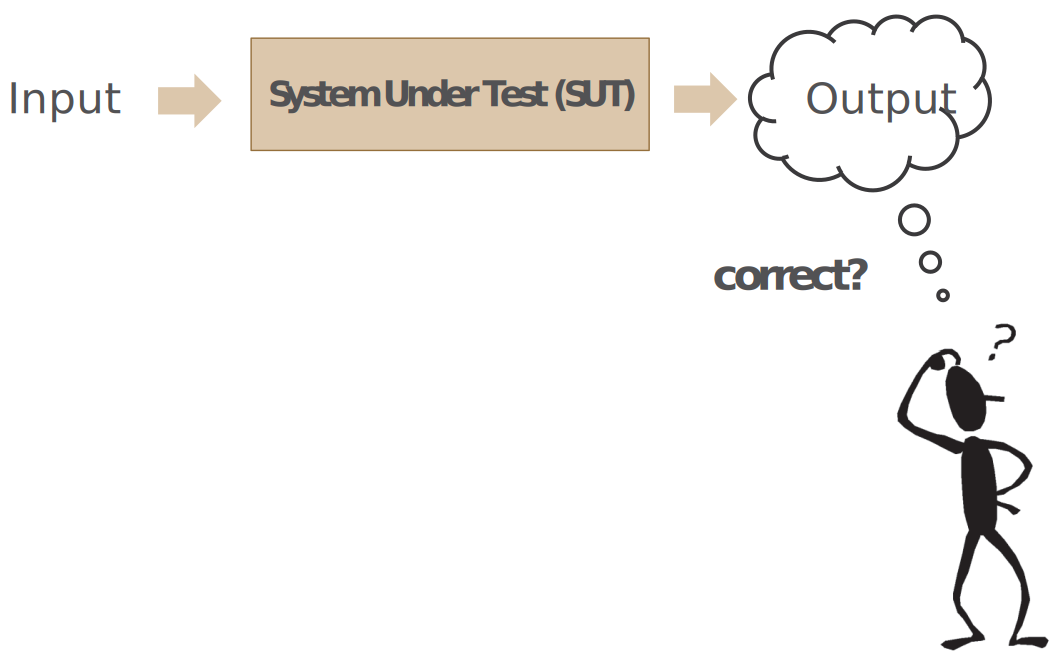
\includegraphics[width=\textwidth]{Qualitaetssicherung/abbildungen/TestOracle}
  \end{center}
\end{frame}

%%%%%%%%%%%%%%%%%%%%%%%%%%%%%%%%%

\begin{frame}
\frametitle{F�r welche Art von Software gibt es keine Test-Orakel?}
  \begin{center}
  \url{https://monti.com}
  \end{center}
\end{frame}

%%%%%%%%%%%%%%%%%%%%%%%%%%%%%%%%%

\begin{frame}
\frametitle{Das Orakel-Problem}
\framesubtitle{Es ist nicht immer m�glich, ein Orakel zu definieren}
  \begin{center}
\only<beamer>{\includegraphics[width=\textwidth]{Qualitaetssicherung/abbildungen/TestOracleProblem}}
  \end{center}
	Was tun? \\
	\citet{MetamorphicTesting2016,segura_metamorphic_2020,kanewala_metamorphic_2019}
\end{frame}

%%%%%%%%%%%%%%%%%%%%%%%%%%%%%%%%%

\begin{frame}
\frametitle{Anwendungsbereiche f�r metamorphisches Testen}
\framesubtitle{\citet{segura_metamorphic_2020}}
  \begin{center}
\only<beamer>{\includegraphics[width=.65\textwidth]{Qualitaetssicherung/abbildungen/MetamorphicTesting}}
  \end{center}
\end{frame}


\mysubsubsection{Integrationstest}

%%%%%%%%%%%%%%%%%%%%%%%%%%%%%%%%%

\begin{frame}
\frametitle{Integrationstest}
\framesubtitle{Testing in the large}
\begin{itemize}
  \item Der Test einzelner Module garantiert nicht, dass die Zusammenarbeit korrekt funktioniert.
  \item Viele Module k�nnen gar nicht isoliert getestet werden.
  \item Also: Vorgehensweise zum Test komplexer Systeme (modulares Testen):
    \begin{itemize}
      \item Modultests (a.k.a.\ Unit Tests \&\ Components Tests)\\
			Testen eine Komponente ohne Kontext.
      \item Inkrementeller Integrationstest mehrer Komponenten im Kontext.
      \item Systemtest: Test des gesamten Systems in der Anwendungsumgebung (end-to-end).
    \end{itemize}
	\item Akzeptanztests (a.k.a.\ Funktionstests)\\
Focus auf das Testen von `cross-cutting' Funktionalit�t.
\end{itemize}
\end{frame}

%%%%%%%%%%%%%%%%%%%%%%%%%%%%%%%%%

\begin{frame}
\frametitle{Integrationstest (Forts.)}
\begin{itemize}
  \item Bei eingebetteten Realzeitsystemen muss auch das Zusammenspiel von Hard- und Software getestet werden.
	\begin{itemize}
		\item Digital Twins
	\end{itemize}
  \item Inkrementelles Testen ist dem \glq Big-Bang\grq-Testen, wobei nach den Modultests direkt das Gesamtsystem getestet wird, vorzuziehen.
  \item Die Trennung zwischen Schnittstelle und Implementierung erleichtert den Integrationstest erheblich.
    \begin{itemize}
      \item Leichtes Ersetzen von \glq Mockups\grq\ durch \glq richtige\grq\ Module.\\
			Siehe z.B.\ Mockito \url{https://github.com/mockito/}
    \end{itemize}
\end{itemize}
\end{frame}

%%%%%%%%%%%%%%%%%%%%%%%%%%%%%%%%%

\begin{frame}
\frametitle{Inkrementelles Testen}
\begin{center}
\pgfimage[width=0.9\textwidth]{Qualitaetssicherung/abbildungen/Inkrementelles_Testen}\\
"`Testger�st"'
\end{center}
 
\begin{itemize}
	\item Inkrementelle Tests k�nnen entsprechend den Benutzt- und Kompositions-Hierarchien bottom-up oder top-down erfolgen; nat�rlich auch jo-jo. 
	\item Eine hierarchische Architektur ist dabei sehr f�rderlich.
\end{itemize}
\end{frame}

\mysubsubsection{Regression testing }

%%%%%%%%%%%%%%%%%%%%%%%%%%%%%%%%%

\begin{frame}
\frametitle{Regression testing}
\begin{itemize}
  \item A test tool saves all test cases that have been done.
  \item This allows for an automatic repretition of all past tests after the software under test was changed.
  \item Executes nominal-actual comparison:
    \begin{itemize}
      \item Input data for the test object
      \item Expected outputs or reactions of test object
    \end{itemize}
\end{itemize}
\end{frame}

%%%%%%%%%%%%%%%%%%%%%%%%%%%%%%%%%

%\begin{frame}
%\frametitle{Test Driven Development}
%\framesubtitle{Testgetriebene Entwicklung}
    %\begin{itemize}
    %\item Martin Fowler:\\
        %``Whenever you are tempted to type something into a print statement or a debugger expression, write it as a test instead.''
    %\item ``One of the ironies of Test Driven Development is that it isn't a testing technique. It's an analysis technique, a design technique, really a technique structuring all the activities of development.'' \cite{Beck2002}.                  
          %
    %\item Testen als Spezifikation und Entwurfsmittel.
          %
    %\item Tests sind eine Form von ausf�hrbarer Dokumentation.
          %
    %\item Regressionstests sind ein n�tzlicher Nebeneffekt.
          %
    %\end{itemize}
%\end{frame}

%%%%%%%%%%%%%%%%%%%%%%%%%%%%%%%%%

%\begin{frame}
%\frametitle{Werkzeugunterst�tzung zum Testen}
%\framesubtitle{Unit- und Integrations-Tests}
%\begin{itemize}
  %\item JUnit ist ein Testwerkzeug f�r Java \citep{Link2002}\\
    %(\url{http://www.junit.org/}).
	%\item Selenium-Integrations-Tests f�r Browser (\url{http://seleniumhq.org/}).
	%\item testIT WebTester als UI-Testautomatisierungs-Framework f�r Web-Applikationen basierend auf Selenium (\url{https://www.novatec-gmbh.de/produkte/testit-webtester/}).
%\end{itemize}
%Unit-Tests und Integrations-Tests sind mit diesen Werkzeugen automatisch wiederholbar.
%\end{frame}

%%%%%%%%%%%%%%%%%%%%%%%%%%%%%%%%%

%\begin{frame}
%\frametitle{Automatisierte Akzeptanztests}
%\framesubtitle{\citep{FIT2005,FIT2006}}
%\begin{itemize}
  %\item Die zu pr�fende Gesch�ftslogik und die erwarteten
    %Testergebnisse werden in Tabellenform dargestellt (HTML), so dass auch
    %Fachexperten an der Erstellung und Durchf�hrung der Tests
    %teilnehmen k�nnen.
  %\item FIT (Framework for Integrated Test) ist ein Werkzeug,
    %welches automatisierte und wiederholbare Akzeptanztests erlaubt
    %(\url{http://fit.c2.com/})
	%\item FitNesse erg�nzt FIT u.a.\ um ein Wiki zur kollaborativen Erstellung von Akzeptanztests (\url{http://www.fitnesse.org/})
%\end{itemize}
%\end{frame}

%%%%%%%%%%%%%%%%%%%%%%%%%%%%%%%%%

\begin{frame}
\frametitle{Test driven development and refactoring}
\begin{itemize}
  \item Test driven development combines two techniques: 
    \begin{itemize}
      \item Test-driven programming for external evolution,
      \item refactoring for internal evolution.
    \end{itemize}
  \item Refactoring\\
        Changing a program with the aim of improving the internal structure without changing the (external) functionality.
  \item Refactoring is allowed if all tests are passing.
  \item Here, tests are a form of executable specification.
\end{itemize}
\end{frame}

%%%%%%%%%%%%%%%%%%%%%%%%%%%%%%%%%

\begin{frame}
\frametitle{Continuous Integration}
Aims for (among others):
\begin{itemize}
	\item Execution of static analyses (e.g., SpotBugs, Checkstyle)
	\item Building the systems (e.g., Gradle)
	\item Automated execution of tests (e.g.\ JUnit, Selenium) \citep{TestAutomation2013}
	\item Checking of log and monitoring data (e.g.\ Kieker) \citep{SEN2015}
\end{itemize}
\end{frame}

%%%%%%%%%%%%%%%%%%%%%%%%%%%%%%%%%

\begin{frame}
\frametitle{DevOps: Development and operations}
\framesubtitle{Continuous Testing, Delivery \&\ Deployment}
\begin{center}
\pgfimage[width=0.7\textwidth]{Qualitaetssicherung/abbildungen/DevOps2016}
\end{center}
\end{frame}

%%%%%%%%%%%%%%%%%%%%%%%%%%%%%%%%%

\begin{frame}
\frametitle{Agility and reliability}
\framesubtitle{By Continuous Testing, Example otto.de \citep{ICSA2017}}
\begin{center}
\pgfimage[width=\textwidth]{Qualitaetssicherung/abbildungen/DeploymentIncidentsBars}
\end{center}
\end{frame}


%%
%\backupbegin
%\section{References}

%%%%%%%%%%%%%%%%%%%%%%%%%%%%%%%%%
%\begin{frame}[t,allowframebreaks]{References}
%  \frametitle{\bibname}
%  \printbibliography
%\end{frame}

%\backupend

\end{document}
